\section{Pianificazione}
Sulla base delle scadenze fissate in §1.6, la ripartizione delle attività di progetto avviene tramite:
\begin{itemize}
\item \textbf{Analisi};
\item \textbf{Consolidamento requisiti};
\item \textbf{Progettazione e codifica per la Technology Baseline};
\item \textbf{Progettazione di dettaglio e codifica};
\item \textbf{Validazione e collaudo}.
\end{itemize}  
Le attività presenti sono una mera descrizione di ciò che bisognerà fare in ogni diversa fase del progetto, pertanto non vengono indicate nella \S 5. Quest'ultima si concentra sulla pianificazione generale dell'intero periodo, senza definire ogni attività, e sugli incrementi apportati al prodotto software.

\subsection{Analisi}
\textit{Periodo: da 2020-03-16 a 2020-04-13} \\
Durante questo periodo il \textit{TeamAFK} si occuperà principalmente dell’analisi di tutte le informazioni riguardanti il prodotto che deve sviluppare, l’organizzazione delle attività e la suddivisione delle risorse.

\subsubsection{Ruoli attivi} 
\begin{itemize}
\item \textit{Responsabile di Progetto};
\item \textit{Amministratore};
\item \textit{Analista};
\item \textit{Progettista};
\item \textit{Verificatore}.
\end{itemize}

\subsubsection{Attività}
\begin{itemize}
\item \textbf{Identificazione degli strumenti}: attività rivolta a determinare gli strumenti da utilizzare per le comunicazioni, stesura dei documenti, versionamento, sviluppo e verifica del sistema;
\item \textbf{Norme di Progetto}: sono l'insieme delle regole da seguire per lo svolgimento dei processi e la realizzazione del prodotto. Il documento \textit{Norme di Progetto} è redatto dall'\textit{Amministratore};
\item \textbf{Studio di Fattibilità}: attività svolta dagli \textit{Analisti} con lo scopo di analizzare i capitolati in linea generale per stabilire quale di essi sia una proposta realizzabile. Inoltre è un'attività propedeutica all'\textit{Analisi dei Requisiti};
\item \textbf{Analisi dei Requisiti}: sulla base dell'attività precedente, vengono identificati e definiti i requisiti del sistema. Come per il documento \textit{Studio di Fattibilità}, anche \textit{Analisi dei Requisiti} viene redatto dagli \textit{Analisti};
\item \textbf{Piano di Qualifica}: attività dell'\textit{Amministratore} e del \textit{Progettista} che si occupa di stabilire le metodologie per garantire la qualità del prodotto. In particolar modo la seconda figura si focalizza sulla parte programmatica;
\item \textbf{Piano di Progetto}: il lavoro da svolgere viene suddiviso in compiti, risorse e attività da parte del \textit{Responsabile} che ha anche il compito di calcolare il preventivo di periodo del progetto. Il tutto viene riportato sempre da parte del \textit{Responsabile} nel documento \textit{Piano di Progetto};
\item \textbf{Glossario}: tutti i vocaboli di difficile interpretazione vengono individuati e riportati nel documento \textit{Glossario}.
\end{itemize}

\begin{figure}[H]
\centering
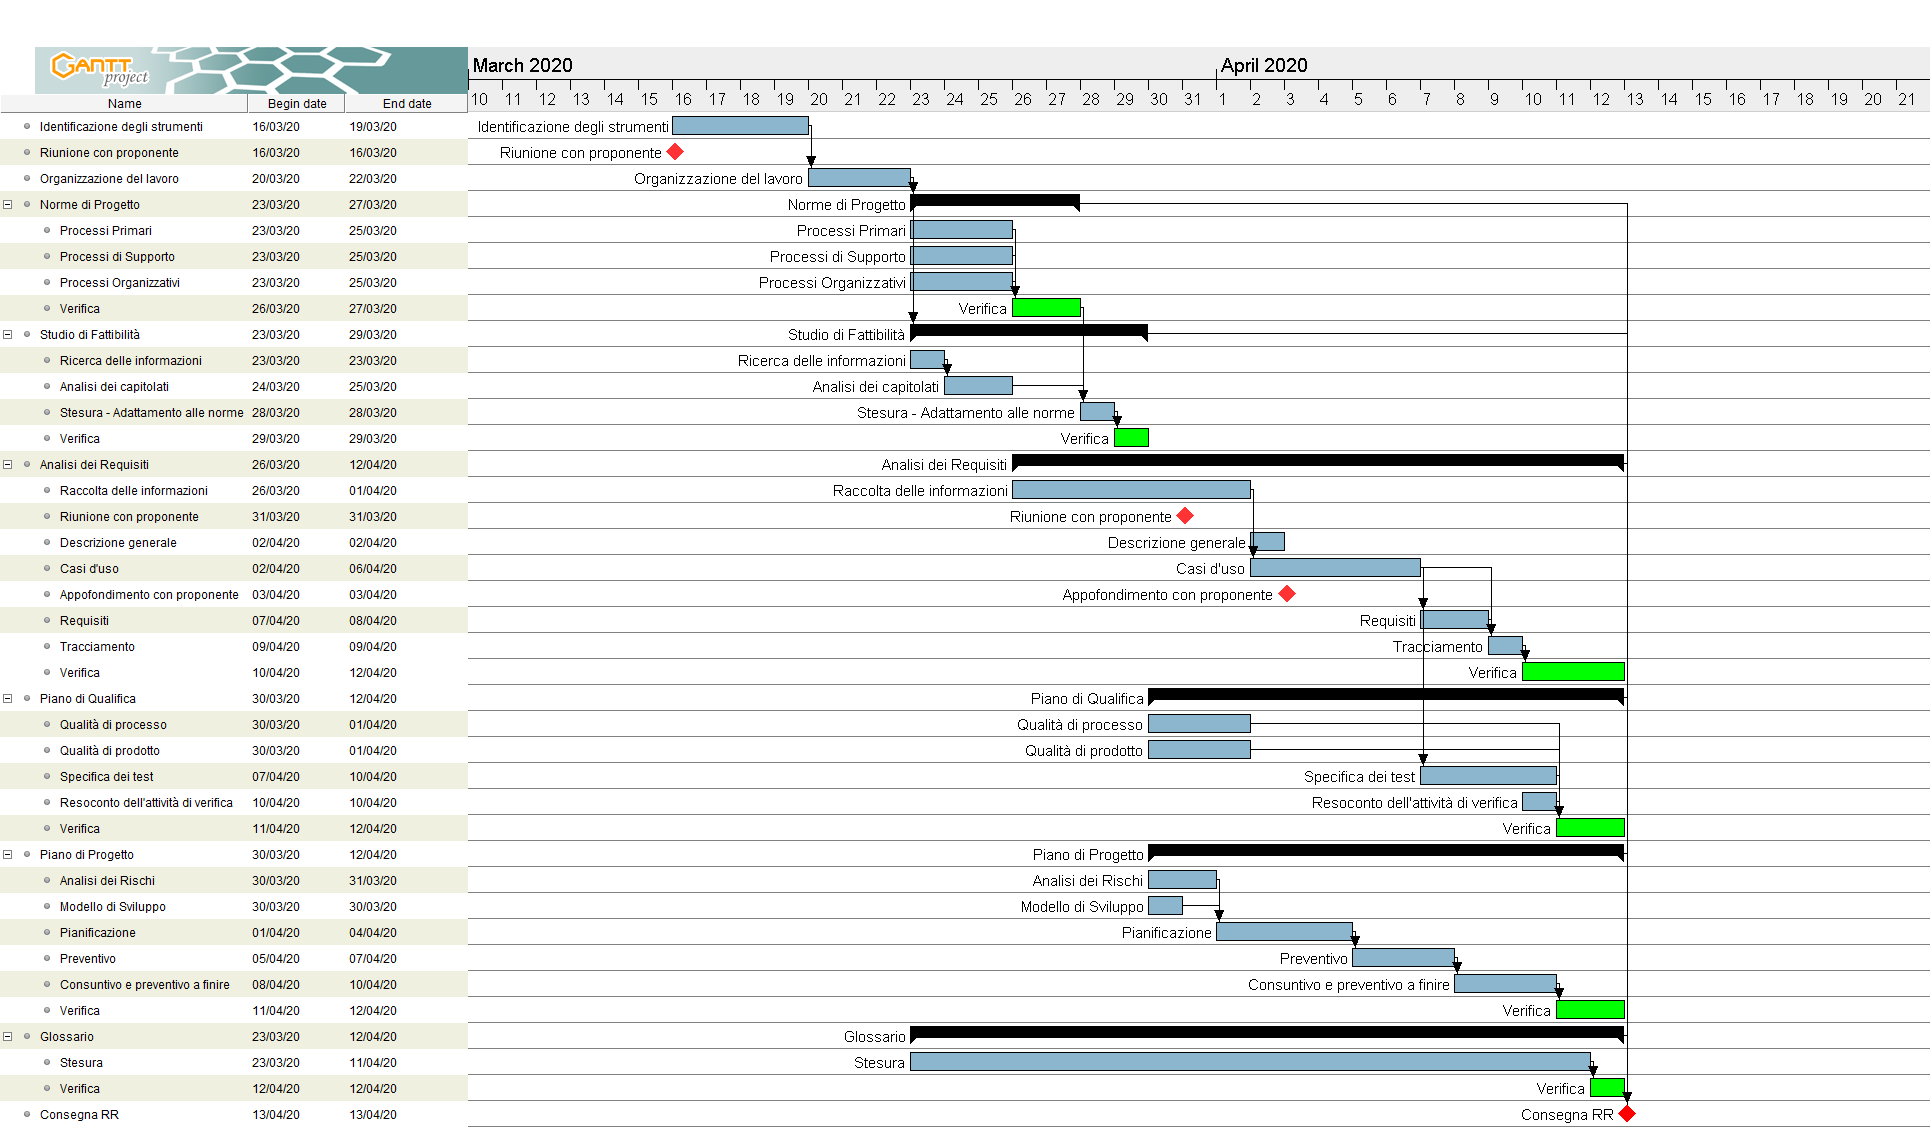
\includegraphics[scale=0.24]{./img/gantt/analisi.png}
\caption{Diagramma di Gantt della fase di Analisi}
\end{figure}

\subsection{Consolidamento dei requisiti}
\textit{Periodo: da 2020-04-14 a 2020-04-20}\\
La fase di consolidamento è così suddivisa:
\begin{itemize}
\item \textbf{Approfondimento personale}: attività intenta a fissare ed approfondire le informazioni riguardanti i requisiti evidenziati nella precedente fase;
\item \textbf{Raccolta informazioni}: raccolta delle informazioni necessarie per la presentazione;
\item \textbf{Stesura presentazione}: preparazione del materiale necessario alla presentazione del 2020-04-20;
\item \textbf{Studio personale}: tempo dedicato ai membri del gruppo, per studiare le informazioni contenute nella presentazione.
\end{itemize}

\begin{figure}[H]
\centering
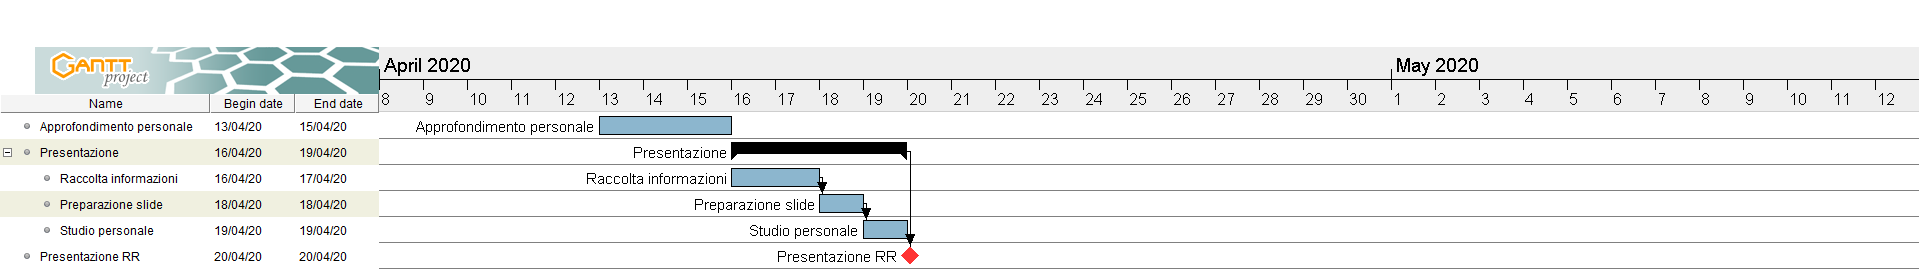
\includegraphics[scale=0.24]{./img/gantt/consolidamento_requisiti.png}
\caption{Diagramma di Gantt della fase di Consolidamento dei requisiti}
\end{figure}

\subsection{Progettazione e codifica per la Technology Baseline}
\textit{Periodo: da 2020-04-21 a 2020-05-11}\\
Questa fase coincide con il giorno successivo alla presentazione del 2020-04-20 e termina con la consegna del materiale per la \textbf{Revisone di Progettazione}.

\subsubsection{Ruoli attivi} \begin{itemize}
\item \textit{Responsabile di Progetto};
\item \textit{Amministratore};
\item \textit{Analista};
\item \textit{Progettista};
\item \textit{Programmatore};
\item \textit{Verificatore}.
\end{itemize}

\subsubsection{Attività}
\begin{itemize}
\item \textbf{Incrementi e verifica dei documenti}: sulla base dei feedback del committente e del proponente, viene migliorato e verificato il materiale del precedente rilascio;
\item \textbf{Progettazione e codifica della Proof of Concept}: vengono identificati i design pattern\glo necessari allo sviluppo del sistema e verranno riportati nell'allegato tecnico insieme al tracciamento dei requisiti. Inoltre viene presentato, al committente e al proponente, un prototipo per mezzo di un repository\glo. In questo periodo saranno implementati solo una parte di requisiti, ovvero quelli che ricoprono le funzionalità del tool di addestramento. La scrittura del codice per lo sviluppo di tali requisiti segue le indicazioni definite nel documento \textit{Norme di Progetto};
\item \textbf{Verifica della Proof of Concept}: vengono testati e verificati tutti gli incrementi sviluppati;
\item \textbf{Preparazione della presentazione}: vengono create le slide da utilizzare per la presentazione della PoC, fissata in data 2020/05/05.
\end{itemize}

\paragraph{Incremento 1}\mbox{} \\ \mbox{} \\ 
\textit{Periodo: da 2020/04/21 a 2020/04/30}\\
L’incremento 1 prevede lo sviluppo e l’implementazione del tool di addestramento, per ottenere il file JSON contenente i predittori. Per sviluppare questo incremento verrà utilizzata la libreria di JS \texttt{JSON.stringify}. \\
Verrà quindi implementata una pagina web che consentirà di: \begin{itemize}
\item caricare il file CSV contenente i dati per l'addestramento;
\item selezionare l'algoritmo di predizione desiderato;
\begin{itemize}
\item nel caso in cui l’utente selezioni un algoritmo incompatibile con il file CSV caricato, sarà mostrato il messaggio di errore "File CSV incompatibile";
\item nel caso in cui l'utente selezioni l'algoritmo senza aver caricato il file CSV, sarà mostrato il messaggio di errore "File CSV non inserito";
\end{itemize}
\item confermare tale algoritmo, per procedere con l'addestramento;
\begin{itemize}
\item l’utente visualizza il messaggio di notifica "Addestramento avvenuto successo", in cui viene notificato che l’addestramento confermato dell’algoritmo selezionato,a partire dai dati di addestramento, è avvenuto correttamente;
\end{itemize}
\item scaricare il file JSON contenente i predittori.
\end{itemize}
Lo sviluppo di questo incremento prevede il soddisfacimento completo dei seguenti requisiti funzionali:
\begin{itemize}
\item Re1F1;
\item Re1F1.1;
\item Re1F1.2;
\item Re1F1.3;
\item Re2F1.6;
\item Re2F1.7;
\item Re1F13.
\end{itemize}
\paragraph*{Verifica}\mbox{} \\ \mbox{} \\ 
\textit{Periodo: da 2020/05/01 a 2020/05/04}\\
Durante questo periodo verranno testate e verificate tutte le funzionalità di questo incremento. Qualora dovessero presentarsi dei bug\glo, sarà compito dei programmatori risolverli nel più breve tempo possibile.

\paragraph{Incremento 2}\mbox{} \\ \mbox{} \\ 
\textit{Periodo: da 2020/04/21 a 2020/04/30}\\
L’incremento 2 prevede lo sviluppo e l’implementazione dell'algoritmo che permette l'inserimento del file JSON, contenente i predittori, nel plug-in. Verrà usato React in sinergia con gli strumenti di sviluppo di plug-in offerti dalla piattaforma Grafana. \\
Sarà quindi possibile:
\begin{itemize}
	\item selezionare il file json da caricare, presente nel file system;
	\item confermare la selezione.
\end{itemize}
Lo sviluppo di questo incremento prevede il soddisfacimento completo dei seguenti requisiti funzionali:
\begin{itemize}
\item Re1F2;
\item Re1F2.1;
\item Re1F2.2;
\item Re1F2.4.
\end{itemize}
\paragraph*{Verifica}\mbox{} \\ \mbox{} \\ 
\textit{Periodo: da 2020/05/01 a 2020/05/03}\\
Durante questo periodo verranno testate e verificate tutte le funzionalità di questo incremento. Qualora dovessero presentarsi dei bug, sarà compito dei programmatori risolverli nel più breve tempo possibile.

\paragraph{Incremento 3}\mbox{} \\ \mbox{} \\ 
\textit{Periodo: da 2020/04/21 a 2020/04/30}\\
L’incremento 3 prevede lo sviluppo e l’implementazione dell'algoritmo che permette il collegamento del plug-in ad un flusso di dati. Verrà usato React in sinergia con gli strumenti di sviluppo di plug-in offerti dalla piattaforma Grafana. \\
Sarà quindi possibile:
\begin{itemize}
	\item selezionare i predittori;
	\item selezionare la query legata al flusso dei dati.
\end{itemize}
Lo sviluppo di questo incremento prevede il soddisfacimento completo dei seguenti requisiti funzionali:
\begin{itemize}
\item Re1F3.1;
\item Re1F3.2.
\end{itemize}
\paragraph*{Verifica}\mbox{} \\ \mbox{} \\ 
\textit{Periodo: da 2020/05/01 a 2020/05/03}\\
Durante questo periodo verranno testate e verificate tutte le funzionalità di questo incremento. Qualora dovessero presentarsi dei bug, sarà compito dei programmatori risolverli nel più breve tempo possibile.

\begin{figure}[H]
\centering
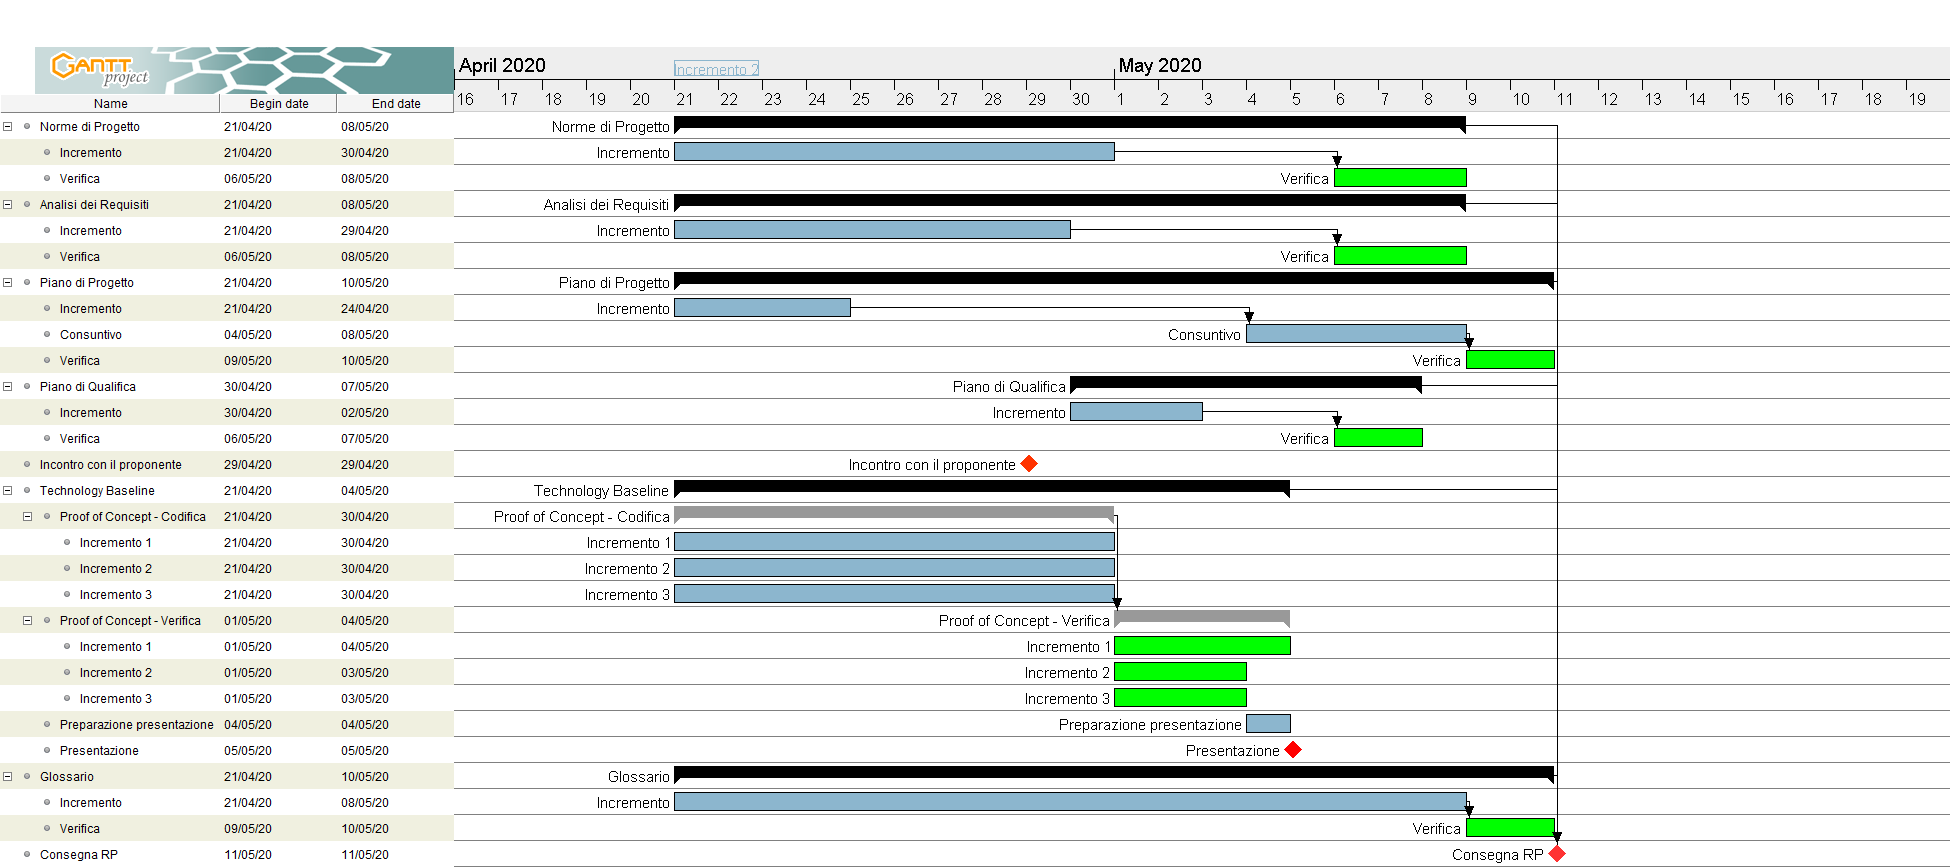
\includegraphics[scale=0.24]{./img/gantt/progettazione_architetturale.png}
\caption{Diagramma di Gantt della fase di Progettazione e codifica per la Technology Baseline}
\end{figure}

\subsection{Progettazine di dettaglio e codifica}
\textit{Periodo: da 2020-05-11 a 2020-06-11}\\
Questa fase è compresa tra il giorno successivo alla presentazione del 2020-05-11 e la consegna della \textit{Revisione di Qualifica}.

\subsubsection{Ruoli attivi} \begin{itemize}
\item \textit{Responsabile di Progetto};
\item \textit{Amministratore};
\item \textit{Analista};
\item \textit{Progettista};
\item \textit{Programmatore};
\item \textit{Verificatore}.
\end{itemize}

\subsubsection{Attività}
\begin{itemize}
\item \textbf{Incrementi e verifica dei documenti}: sulla base dei feedback del committente e del proponente, viene migliorato e verificato il materiale del precedente rilascio;
\item \textbf{Codifica degli incrementi}: 
\item \textbf{Verifica degli incrementi}: 
\item \textbf{Preparazione della presentazione}: vengono create le slide da utilizzare per la presentazione della Product Baseline.
\end{itemize}

\paragraph{Incremento 4}\mbox{} \\ \mbox{} \\ 
\textit{Periodo: da 2020-05-22 a 2020-05-26}\\
L’incremento 4 prevede il completamento dello sviluppo del tool di addestramento, aggiungendo i messaggi di alert mancanti.\\
Sarà quindi possibile:
\begin{itemize}
	\item visualizzare il messaggio di addestramento avvenuto con successo;
	\item visualizzare l'errore di addestramento non riuscito;
	\item visualizzare l'errore CSV non caricato;
	\item visualizzare l'alert algoritmo non scelto. 
\end{itemize}
Lo sviluppo di questo incremento prevede il soddisfacimento completo dei seguenti requisiti funzionali:
\begin{itemize}
\item Re1F1.4;
\item Re2F1.5;
\item Re1F11;
\item Re1F12.
\end{itemize}
\paragraph*{Verifica}\mbox{} \\ \mbox{} \\ 
\textit{Periodo: da 2020-05-27 a 2020-05-28}\\
Durante questo periodo verranno testate e verificate tutte le funzionalità di questo incremento. Qualora dovessero presentarsi dei bug, sarà compito dei programmatori risolverli nel più breve tempo possibile.

\paragraph{Incremento 5}\mbox{} \\ \mbox{} \\ 
\textit{Periodo: da 2020-05-22 a 2020-05-25}\\
L’incremento 5 prevede il completamento dello sviluppo del caricamento del file json nel plug-in, aggiungendo i messaggi di alert mancanti.\\
Sarà quindi possibile:
\begin{itemize}
	\item visualizzare il messaggio di avvenuto caricamento del file json.
\end{itemize}
Lo sviluppo di questo incremento prevede il soddisfacimento completo dei seguenti requisiti funzionali:
\begin{itemize}
\item Re2F2.3.
\end{itemize}
\paragraph*{Verifica}\mbox{} \\ \mbox{} \\ 
\textit{Periodo: da 2020-05-26 a 2020-05-27}\\
Durante questo periodo verranno testate e verificate tutte le funzionalità di questo incremento. Qualora dovessero presentarsi dei bug, sarà compito dei programmatori risolverli nel più breve tempo possibile.

\paragraph{Incremento 6}\mbox{} \\ \mbox{} \\ 
\textit{Periodo: da 2020-05-23 a 2020-05-27}\\
L’incremento 6 prevede l'inserimento del collegamento e la visualizzazione della lista dei predittori collegati. \\
Sarà quindi possibile:
\begin{itemize}
	\item confermare le impostazioni di collegamento;
	\item visualizzare la lista dei predittori precedentemente collegati.
\end{itemize}
Lo sviluppo di questo incremento prevede il soddisfacimento completo dei seguenti requisiti funzionali:
\begin{itemize}
\item Re1F3.5;
\item Re1F4.
\end{itemize}
\paragraph*{Verifica}\mbox{} \\ \mbox{} \\ 
\textit{Periodo: da 2020-05-30 a 2020-05-30}\\
Durante questo periodo verranno testate e verificate tutte le funzionalità di questo incremento. Qualora dovessero presentarsi dei bug, sarà compito dei programmatori risolverli nel più breve tempo possibile.

\paragraph{Incremento 7}\mbox{} \\ \mbox{} \\ 
\textit{Periodo: da 2020-05-28 a 2020-05-29}\\
L’incremento 7 prevede il completamente del pannello di collegamento. \\
Sarà quindi possibile:
\begin{itemize}
	\item collegare il predittore al flusso dati;
	\item aggiungere il nome ad un collegamento.
\end{itemize}
Lo sviluppo di questo incremento prevede il soddisfacimento completo dei seguenti requisiti funzionali:
\begin{itemize}
\item Re1F3;
\item Re1F3.4.
\end{itemize}
\paragraph*{Verifica}\mbox{} \\ \mbox{} \\ 
\textit{Periodo: da 2020-05-30 a 2020-05-30}\\
Durante questo periodo verranno testate e verificate tutte le funzionalità di questo incremento. Qualora dovessero presentarsi dei bug, sarà compito dei programmatori risolverli nel più breve tempo possibile.

\paragraph{Incremento 8}\mbox{} \\ \mbox{} \\ 
\textit{Periodo: da 2020-05-28 a 2020-05-30}\\
L’incremento 8 prevede lo sviluppo della funzionalità di scollegamento dei predittori.\\
Sarà quindi possibile:
\begin{itemize}
	\item scollegare il/i predittore/i;
	\item visualizzare il messaggio di conferma del scollegamento;
	\item selezionare se confermare o annullare lo scollegamento;
	\item visualizzare il messaggio di avvenuto scollegamento.
\end{itemize}
Lo sviluppo di questo incremento prevede il soddisfacimento completo dei seguenti requisiti funzionali:
\begin{itemize}
\item Re1F5;
\item Re1F5.1;
\item Re1F5.2;
\item Re1F5.3;
\item Re2F5.4;
\item Re1F5.5.
\end{itemize}
\paragraph*{Verifica}\mbox{} \\ \mbox{} \\ 
\textit{Periodo: da 2020-05-31 a 2020-05-31}\\
Durante questo periodo verranno testate e verificate tutte le funzionalità di questo incremento. Qualora dovessero presentarsi dei bug, sarà compito dei programmatori risolverli nel più breve tempo possibile.

\paragraph{Incremento 9}\mbox{} \\ \mbox{} \\ 
\textit{Periodo: da 2020-05-28 a 2020-06-01}\\
L’incremento 9 prevede lo sviluppo della funzionalità di modifica dei predittori. \\
Sarà quindi possibile:
\begin{itemize}
	\item modificare il nome del collegamento;
	\item modificare il flusso di dati associato al collegamento;
	\item salvare/annullare le modifiche effettuate;
	\item visualizzare i messaggi di alert/errori dedicati.
\end{itemize}
Lo sviluppo di questo incremento prevede il soddisfacimento completo dei seguenti requisiti funzionali:
\begin{itemize}
\item Re1F6;
\item Re1F6.1;
\item Re1F6.2;
\item Re1F6.3;
\item Re2F6.4;
\item Re1F6.5.
\end{itemize}
\paragraph*{Verifica}\mbox{} \\ \mbox{} \\ 
\textit{Periodo: da 2020-06-01 a 2020-06-03}\\
Durante questo periodo verranno testate e verificate tutte le funzionalità di questo incremento. Qualora dovessero presentarsi dei bug, sarà compito dei programmatori risolverli nel più breve tempo possibile.

\paragraph{Incremento 10}\mbox{} \\ \mbox{} \\ 
\textit{Periodo: da 2020-06-01 a 2020-06-02}\\
L’incremento 10 prevede lo sviluppo della funzionalità di monitoraggio delle previsioni. \\
Sarà quindi possibile:
\begin{itemize}
	\item avviare il monitoraggio;
	\item visualizzare il messaggio di conferma di avvio corretto del monitoraggio.
\end{itemize}
Lo sviluppo di questo incremento prevede il soddisfacimento completo dei seguenti requisiti funzionali:
\begin{itemize}
\item Re1F7;
\item Re1F7.1;
\item Re2F7.2.
\end{itemize}
\paragraph*{Verifica}\mbox{} \\ \mbox{} \\ 
\textit{Periodo: da 2020-06-03 a 2020-06-03}\\
Durante questo periodo verranno testate e verificate tutte le funzionalità di questo incremento. Qualora dovessero presentarsi dei bug, sarà compito dei programmatori risolverli nel più breve tempo possibile.

\paragraph{Incremento 11}\mbox{} \\ \mbox{} \\ 
\textit{Periodo: da 2020-05-30 a 2020-05-31}\\
L’incremento 11 prevede lo sviluppo del collegamento al database per il salvataggio delle previsioni. Per poter svolgere questo incremento è necessario l'aver implementato il calcolo delle previsioni. \\
Sarà quindi possibile:
\begin{itemize}
	\item salvare le previsione nel database;
	\item selezionare il datasource;
	\item assegnare un nome alla tabella;
	\item abilitare/disabilitare il salvataggio;
	\item visualizzare il messaggio di conferma/errore dedicati.
\end{itemize}
Lo sviluppo di questo incremento prevede il soddisfacimento completo dei seguenti requisiti funzionali:
\begin{itemize}
\item Re1F8;
\item Re1F8.1;
\item Re1F8.2;
\item Re1F8.3;
\item Re2F8.4;
\item Re1F8.5;
\item Re2F8.6.
\end{itemize}
\paragraph*{Verifica}\mbox{} \\ \mbox{} \\ 
\textit{Periodo: da 2020-06-01 a 2020-06-01}\\
Durante questo periodo verranno testate e verificate tutte le funzionalità di questo incremento. Qualora dovessero presentarsi dei bug, sarà compito dei programmatori risolverli nel più breve tempo possibile.

\paragraph{Incremento 12}\mbox{} \\ \mbox{} \\ 
\textit{Periodo: da 2020-06-01 a 2020-06-03}\\
L’incremento 12 prevede la visualizzazione della dashboard nella lista dei plug-in disponibili di Grafana. \\
Sarà quindi possibile:
\begin{itemize}
	\item visualizzare la dashboard del plug-in.
\end{itemize}
Lo sviluppo di questo incremento prevede il soddisfacimento completo dei seguenti requisiti funzionali:
\begin{itemize}
\item Re1F10;
\item Re1F10.1.
\end{itemize}
\paragraph*{Verifica}\mbox{} \\ \mbox{} \\ 
\textit{Periodo: da 2020-06-04 a 2020-06-05}\\
Durante questo periodo verranno testate e verificate tutte le funzionalità di questo incremento. Qualora dovessero presentarsi dei bug, sarà compito dei programmatori risolverli nel più breve tempo possibile.

\begin{figure}[H]
\centering
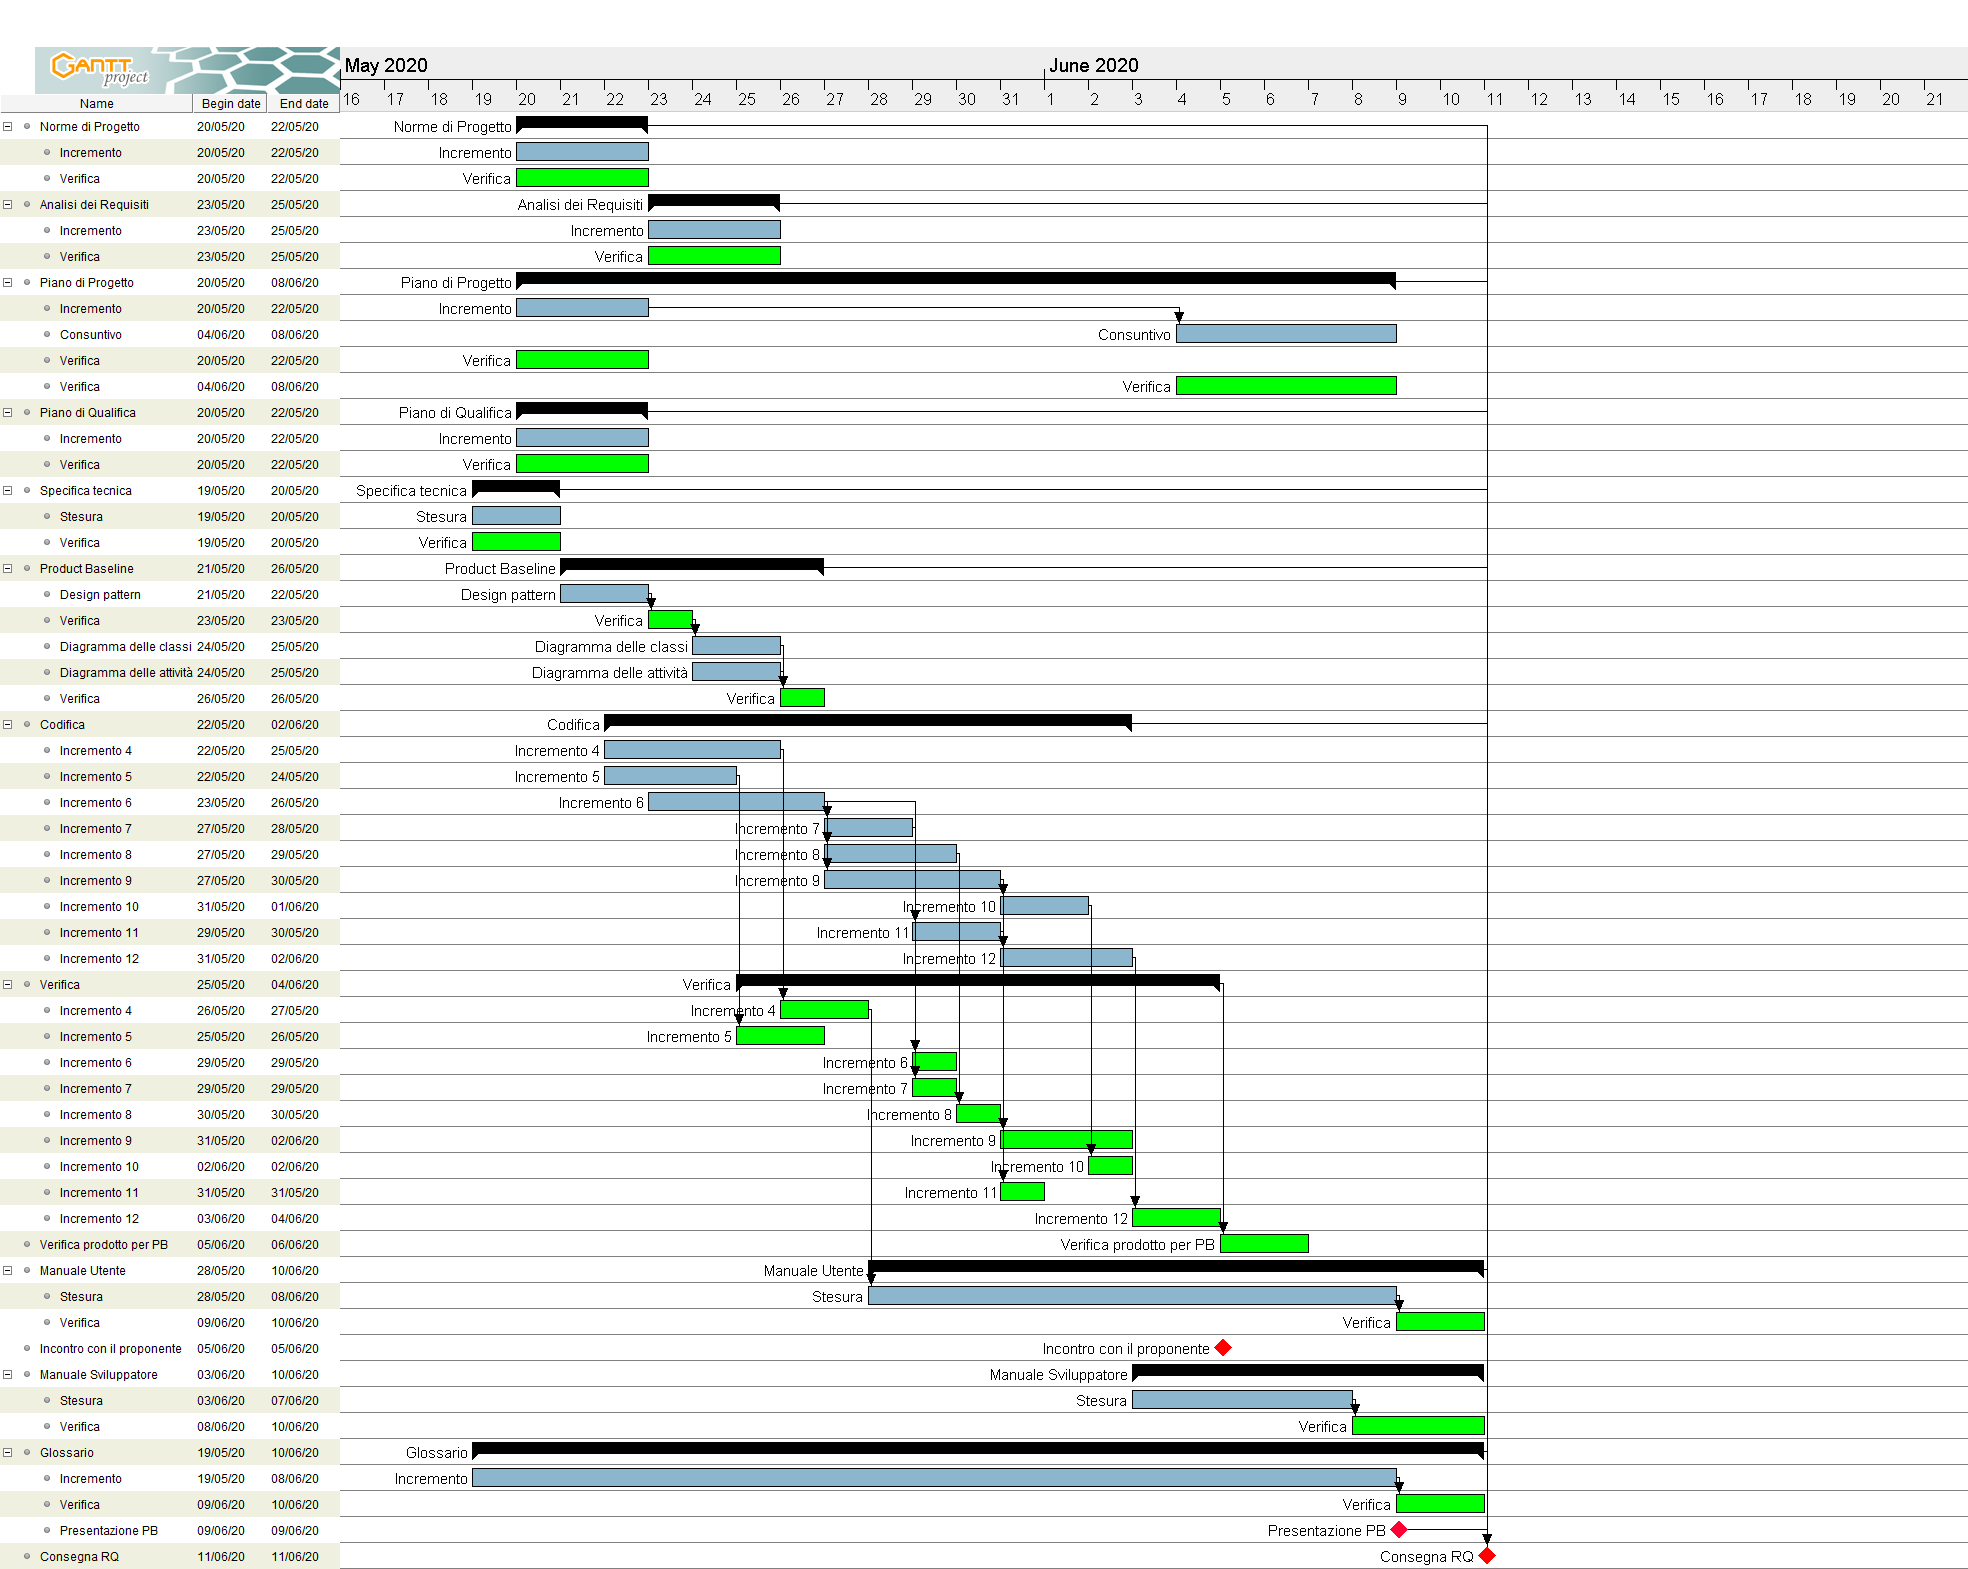
\includegraphics[scale=0.24]{./img/gantt/progettazione_dettaglio_codifica.png}
\caption{Diagramma di Gantt della fase di Progettazione di dettaglio e codifica}
\end{figure}

\subsection{Validazione e collaudo}
\textit{Periodo: da 2020-06-19 a 2020-07-17}\\
La seguente fase inizia il giorno seguente la \textit{Revisione di Qualifica} e termina con la consegna del materiale richiesto per la \textit{Revisione di Accettazione}.

\subsubsection{Ruoli attivi} \begin{itemize}
\item \textit{Responsabile di Progetto};
\item \textit{Amministratore};
\item \textit{Analista};
\item \textit{Progettista};
\item \textit{Programmatore};
\item \textit{Verificatore}.
\end{itemize}

\subsubsection{Attività}
\begin{itemize}
\item \textbf{Codifica degli incrementi}:\\
\textit{Periodo: da 2020-06-22 a 2020-06-26} \\
nel caso risultasse necessario vengono effettuati miglioramenti sulla base di feedback e/o requisiti obbligatori mancanti;
\item \textbf{Validazione e collaudo}: \\
\textit{Periodo: da 2020-06-27 a 2020-07-15} \\
la validazione effettua test sul prodotto, mentre la convalidazione controlla se viene rispettata la coerenza tra il prodotto e le specifiche evidenziate nel documento \textit{Analisi dei Requisiti};
\item \textbf{Manuale Sviluppatore}: viene aggiornato ed incrementato il documento \textit{Manuale dello Sviluppatore}, il quale conterrà le informazioni necessarie allo sviluppo, mantenimento e manutenzione del prodotto;
\item \textbf{Manuale Utente}: viene aggiornato ed incrementato il documento \textit{Manuale dell'Utente}, il quale conterrà le informazioni necessarie all'utilizzo del prodotto.
\end{itemize}

\paragraph{Incremento 13}\mbox{} \\ \mbox{} \\ 
\textit{Periodo: da 2020-06-22 a 2020-06-24} \\
L'incremento 13 prevede lo sviluppo della funzionalità di interruzione del monitoraggio. Sarà quindi possibile: \begin{itemize}
\item interrompere il monitoraggio del flusso dati.
\item visualizzare i messaggi di conferma/errore dedicati.
\end{itemize}
Lo sviluppo di questo incremento prevede il soddisfacimento completo dei seguenti requisiti funzionali: \begin{itemize}
\item Re1F9;
\item Re1F9.1;
\item Re2F9.2.
\end{itemize}

\paragraph{Incremento 14}\mbox{} \\ \mbox{} \\ 
\textit{Periodo: da 2020-06-25 a 2020-06-26}\\
L'incremento 14 prevede l'inserimento di messaggi di notifica/errori mancanti nel plug-in. Sarà quindi possibile visualizzare: \begin{itemize}
\item visualizzare il messaggio d'errore "Collega tutti i predittori";
\item visualizzare il messaggio d'errore "Inserisci un nome per la connessione";
\item visualizzare il messaggio d'errore "Attenzione! Monitoraggio attivo";
\item visualizzare il messaggio d'errore "Nessun predittore collegato".
\end{itemize}
Lo sviluppo di questo incremento prevede il soddisfacimento completo dei seguenti requisiti funzionali: \begin{itemize}
\item Re1F14;
\item Re1F16;
\item Re1F17;
\item Re1F18.
\end{itemize}

\begin{figure}[H]
\centering
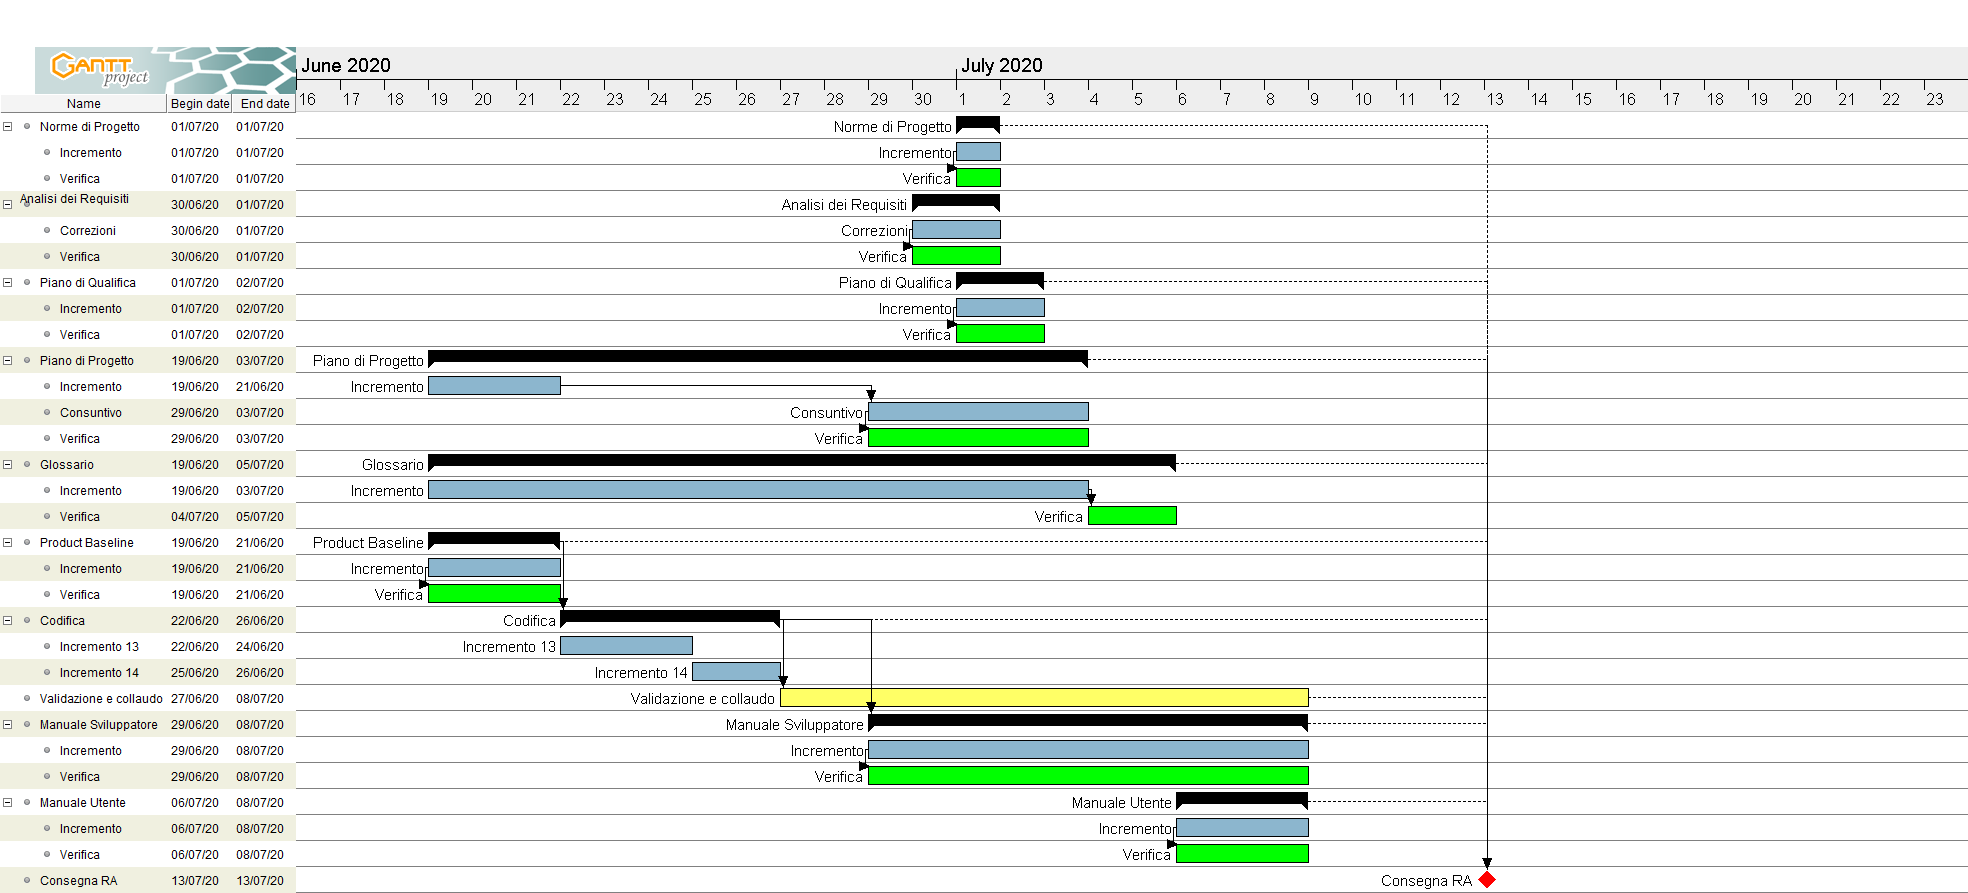
\includegraphics[scale=0.24]{./img/gantt/validazione_collaudo.png}
\caption{Diagramma di Gantt della fase di Validazione e collaudo}
\end{figure}